\documentclass[12pt]{article}
\usepackage[utf8]{inputenc}
\usepackage{tikz}

\begin{document}
    \section*{Aufgabe 1}
\


    Die Induktion wird genutzt, um Definitionen und Beweise durchzuführen.
    \subsection*{Aufgabe Induktive Mengendefinitionen}
    Die Menge

    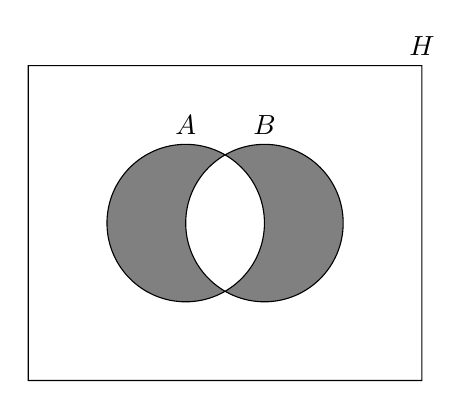
\begin{tikzpicture}[fill=gray]
        % left hand
        \scope
        \clip (-2,-2) rectangle (2,2)
              (1,0) circle (1);
        \fill (0,0) circle (1);
        \endscope
        % right hand
        \scope
        \clip (-2,-2) rectangle (2,2)
              (0,0) circle (1);
        \fill (1,0) circle (1);
        \endscope
        % outline
        \draw (0,0) circle (1) (0,1)  node [text=black,above] {$A$}
              (1,0) circle (1) (1,1)  node [text=black,above] {$B$}
              (-2,-2) rectangle (3,2) node [text=black,above] {$H$};
    \end{tikzpicture}
\end{document}
